\begin{answer}
\begin{center}
    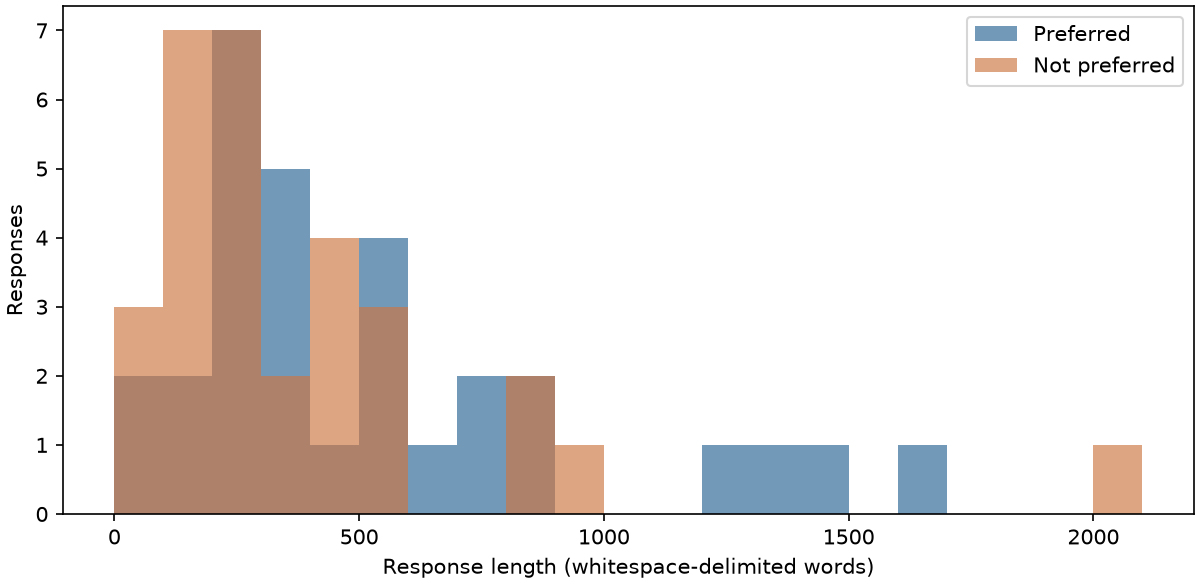
\includegraphics[width=0.85\linewidth]{static/alpaca_lengths_gpt54.png}
\end{center}
Both histograms contain 30 responses and use the same bins. Length is the
number of whitespace-separated words. The median was 374 words for the
preferred answers and 291 for the other answers. Z chose the longer answer
in 23 of 30 pairs, but it chose the shorter answer in the other seven.
E's responses had a median length of 449.5 words, compared with 275.5 for F.

I would treat the 80\% win rate as evidence of what this judge preferred
on these prompts. It does not establish what users generally prefer. Longer
answers sometimes supplied useful details and sometimes made a simple task
harder to start. Since length and content changed together, the histogram
does not show that length alone caused the verdicts. The disagreement in
my five blind comparisons is an additional reason to check the judge
against more human ratings.
\end{answer}
